

\published{Geophysical Journal International, 216, 1214-1232, (2019)}
  
\title{Deblending of simultaneous-source data using a structure-oriented space-varying median filter}
\renewcommand{\thefootnote}{\fnsymbol{footnote}}

\author{Yangkang Chen\footnotemark[1], Shaohuan Zu\footnotemark[2]\footnotemark[3], Yufeng Wang\footnotemark[3], and Xiaohong Chen\footnotemark[3]}
\address{
\footnotemark[1]
School of Earth Sciences\\
Zhejiang University\\
Hangzhou, Zhejiang Province, China, 310027\\
chenyk2016@gmail.com\\
\footnotemark[2] Modeling and Imaging Laboratory\\
Earth and Planetary Sciences\\
University of California\\
Santa Cruz, CA 95064\\
zushaohuan@qq.com\\
\footnotemark[3]State Key Laboratory of Petroleum Resources and Prospecting \\
China University of Petroleum \\
Fuxue Road 18th\\
Beijing, China, 102200 \\
hellowangyf@163.com \& chenxh@cup.edu.cn \\
}

\lefthead{Chen et al.}
\righthead{SOSVMF}

\DeclareRobustCommand{\dlo}[1]{}
\DeclareRobustCommand{\wen}[1]{#1}


\begin{abstract}
In seismic data processing, the median filter\dlo{ (MF)} is usually applied along the structural direction of seismic data in order to attenuate erratic or spike-like noise. The performance of a structure-oriented median filter\dlo{ (SOMF)} highly depends on the accuracy of \new{the} estimated local slope from the noisy data. When local slope contains significant error, which is usually the case for noisy data, the \dlo{SOMF}\wen{structure-oriented median filter} will still cause severe damages to useful energy. \dlo{In this paper, we}\wen{We} propose a type of \dlo{SOMF}\wen{structure-oriented median filter} that can effectively attenuate spike-like noise even when the local slope is not accurately estimated, which we call \dlo{SOSVMF}\wen{structure-oriented space-varying median filter}. \wen{A structure-oriented space-varying median filter} can adaptively squeeze and stretch the window length of the \dlo{MF }\wen{median filter }when applied in the locally flattened dimension of an input seismic data in order to deal with the dipping events caused by inaccurate slope estimation. We show the key difference among different types of median filters in detail and demonstrate the principle of the \dlo{SOSVMF}\wen{structure-oriented space-varying median filter} method. We apply the \dlo{SOSVMF}\wen{structure-oriented space-varying median filter} method to remove the spike-like blending noise arising from the simultaneous source acquisition. Synthetic and real data examples show that \dlo{SOSVMF}\wen{structure-oriented space-varying median filter} can significantly improve the signal preserving performance for curving events in the seismic data. The \dlo{SOSVMF}\wen{structure-oriented space-varying median filter} can also be easily embedded into an iterative deblending procedure based on the shaping regularization framework and can help obtain much improved deblending performance. 
\end{abstract}

\section{Keywords}
Seismic signal processing, noise attenuation, median filter


\maketitle


\section{Introduction}
Simultaneous shooting has been a long-standing research topic in the industry, aiming at boosting the acquisition efficiency by significantly shortening the acquisition time period as well as improving subsurface sampling by increased shot density \cite[]{beasleycj2008,wapenaark2012,abma2014,amundsen2017multi,shaohuan2017jag,asgedom2017rough,zhang2017improving,kim2017efficient,wang2017building,wujuan2018jse1}. Because of the \dlo{much saved}\wen{reduced} acquisition cost, it supports more frequent\dlo{ly periodical} data recording in time-lapse seismic monitoring. Due to the \dlo{tremendously }improved spatial shot sampling, it makes the high-resolution subsurface imaging and inversion more achievable.  All the aforementioned benefits, however, are compromised by the intense \dlo{crosstalk}\wen{interference} noise introduced during simultaneous shooting \cite[]{panagiotis20122,arazthesis2012,qushan2014,sixuethesis2014,sixue2015,yangkang2016irr5d,yatong2018gji,baimin2018jse2,yatong2018dbi,yatong2018jse}. To deal with the strong blending noise in simultaneous source data, one can either develop new algorithms to separate the blended records so that the subsequent processing and workflows do not need to be changed, which is called deblending, or to design new workflows for migrating the blended data directly regardless of the intense interference, which is called direct imaging \cite[]{verschuur2011,shuwei2016vscan,shaohuan2017,baimin2017jse1,wujuan2018cg1,baimin2018cg,baimin2018jse1,qingchen2018gji,qingchen2018tgrs}. 

There are two main types of deblending approaches. The first is based on filtering, which simply treats the blending interference as noise and uses denoising algorithms to remove it \cite[]{mostafa2016geo,mostafa2016jag,mostafa2016bssa,mostafa2017geo}. These methods include the median filtering based approaches \cite[]{mediandeblend,yangkang2015svmf,shuwei2016,weilin2018grsl}, adaptive subtraction methods \cite[]{spitz2008,kim2009}, and dip filtering based methods \cite[]{hampson2008}.
The second is based on inversion.  The inversion based algorithms take advantage of iterative solvers to solve the ill-posed inverse problem in deblending.  Regularization strategies should be used to \dlo{guarantee the convergence during iteration}\wen{constrain the model to be the desired solution}. A number of methods based on different types of constraints have been developed in the literature, e.g., the seislet constraint \cite[]{yangkang20142}, the curvelet constraint \cite[]{kumar2015source,qushan2016,shaohuan2016}, the Fourier constraint \cite[]{abma2015}, the rank constraint \cite[]{jinkun2016,yatong2017ieee}, the hybrid rank-sparsity constraint \cite[]{shaohuan2017gji}, and the hybrid mask-sparsity constraint \cite[]{yatong2017pocs}. \wen{Here ``seislet constrint'' denote ``seislet-domain sparsity constraint''. } While the filtering based methods are more computational efficient and easier to implement, the inversion-based approaches usually lead to better deblending performance \cite[]{borselen2012,shaohuan2016}. 

To date, there are also \dlo{a lot of}\wen{many} reported trials for directly migrating the simultaneous source data. Because of the strong \dlo{crosstalk}\wen{interference} noise, the migrated images might contain distinct artifacts if no extra implementation step is introduced into the migration process. \dlo{?  utilized the inversion based migration strategy, i.e., the least-squares migration to suppress the migration artifacts to some extent. To further attenuate the artifacts, they carefully designed a deblurring filter to constrain the least-squares migration to be structurally smooth.} \cite{berkhout2012} discussed the illumination aspect of direct imaging of simultaneous source data. \cite{zhiguang2016} proposed a new direct imaging method that is based on least-squares reverse time migration\dlo{ (LSRTM)} and structural enhancing operator \cite[]{liuyang2010}. Different from the preconditioning constraint that was used in \cite{daiwei2011}, \cite{zhiguang2016} developed a new iterative solver to solve the \dlo{LSRTM}\wen{least-squares reverse time migration} related inverse problem, which is based on the shaping regularization framework. To tackle the smearing problem of structural smoothing operator in the \dlo{LSRTM}\wen{least-squares reverse time migration} method proposed by \cite{zhiguang2016}, \cite{yangkang2017lsrtm} developed a local singular spectrum analysis (SSA) constraint to preserve the edges and discontinuities on the image. While those imaging methods are promising to make the future imaging framework more flexible, most reported successes are stuck on the synthetic test. A lot of researchers are still working hard to push the direct imaging technique from simulation to practical applications \cite[]{dutta2017lsrtm,lichuang2018}. 

In this paper, we are aiming at introducing a novel median filtering method for either separating the simultaneous sources in a fast one-step way, or iteratively improving the traditional shaping regularized deblending approaches by constructing a more powerful shaping operator. Since the new method is \dlo{in}\wen{by} nature a type of median filter, it is worth mentioning some existing\dlo{ ways} \wen{methods} that use median filtering\dlo{ methods} for deblending. \cite{mediandeblend} proposed a multi-dimensional vector median filter for separating \dlo{blended }simultaneous-source data. A dip scanning step is first performed so that a vector median filter can be applied along the structural direction. \cite{yangkang2015svmf} developed a space-varying median filter to deal with curved events in seismic data. The filter length varies spatially so that noise is removed using a long filter length and the signal is preserved using a relatively smaller filter length. \cite{shuwei2016} proposed a structure-oriented median filter to maximize the effectiveness of a median filter when processing a complicated dataset. Both methods in either \cite{mediandeblend} or \cite{shuwei2016} can be considered as structure-oriented filtering, which requires an sufficiently-accurate slope estimation. However, when the slope is not properly estimated, e.g., in the case of strong ambient noise and blending noise, the structural filtering strategy would fail because those filters will tend to damage signal energy. 

We investigate the reason why the structural filtering fails when the slope is not accurate enough. The principle of the structural filtering is to create a local window along the structural direction, or in other words, to create a locally flattened gather to apply the 1D median or mean filter. When the slope is accurate, e.g., using the plane-wave destruction\dlo{ (PWD)} algorithm \cite[]{fomel2002pwd}, the local gather is exactly flattened. However, when the slope is not precise enough, the local gather still contains curved events. In this case, we take advantage of the \dlo{space varying}\wen{spatially varying} median filter to deal with the slightly curved events in the flattened dimension. The proposed method is thus capable of preserving more useful energy than the traditional structural filtering method.

The paper is organized as follows, we first introduce the basics of median filtering\dlo{ (MF)} and structure-oriented filtering\dlo{ (SOMF)}. Then, we focus on introducing the proposed structure-oriented space-varying median filtering method\dlo{ (SOSVMF)}. We also introduce the way we imbed the proposed filtering method in the shaping regularized iterative deblending framework. Next, we use several synthetic and real data examples to show the potential of the proposed method, either in obtaining a fast simultaneous source separation, or in improving the deblending performance \dlo{through}\wen{in} an iterative fashion. Finally, we draw some key conclusions at the end of the paper.


\section{Structural-oriented space-varying median filter (SOSVMF)}
\subsection{Median filter}
A median filter\dlo{ (MF)} can be used to obtain successful performance in rejecting \dlo{impulse}\wen{impulsive} (spiky) noise, which has \dlo{extreme}\wen{anomalous} value compared with neighboring values. Compared with the commonly known smoothing filter, the median filter enjoys several advantages such as preserving edges, being less sensitive to \dlo{extreme}\wen{anomalous} values and being able to be applied repeatedly. Given a 2D signal, e.g., the waveform\wen{s} recorded by \dlo{Laser Doppler interferometer receiver}\wen{geophone arrays}, a 1D median filter is applied along the spatial direction and each row of the waveform matrix is filtered one by one. Mathematically, a median filter can be expressed using the following formula \cite[]{yangkang2015svmf} when applied to a 2D signal: \dlo{$\hat{u}_{i,j}=\arg\min_{u_m\in U_{i,j}}\sum_{l=1}^{L}\Arrowvert u_m-u_l \Arrowvert_1$}
\wen{\begin{equation}
\label{eq:mf1}
\min_{u_m\in U_{i,j}}\sum_{l=1}^{L}\Arrowvert u_m-u_l \Arrowvert_1,
\end{equation}}
\dlo{where $\hat{u}_{i,j}$ is the}\wen{The solution of minimization problem \ref{eq:mf1} is the} output value for location $x_{i,j}$. $U_{i,j}=\{u_1,u_2,\cdots,u_L\}$ denotes the 1D \dlo{filering}\wen{filtering} window. $i,j$ are the position indices in a 2D profile. $l$ and $m$ are both indices in the filtering window. \wen{Both $u_l$ and $u_m$ are temporary variables.} $L$ is the length of the filtering window. \wen{Simply speaking, for each point in the 2D data, the median filter substitutes it with the median of neighbor points included by the window with size $L$. The process of $\min_{u_m}\sum_{l=1}^{L}\Arrowvert u_m-u_l \Arrowvert_1$ corresponds to finding the median in the window constructed by $\{u_1,u_2,u_3,\cdots,u_L\}$.  }

\subsection{Median filter along the structural direction}
Median filtering has a remarkable capability for attenuating spike-like noise. However, the median filter might still cause some damage\dlo{s} to useful components when the data is highly non-stationary in the space direction. Considering that the recorded waveforms may have structural patterns, if the median filter is applied along the structural direction, the damage can be minimized. We utilize a way that is used in reflection seismic data processing to flatten the recorded waveform data in a local manner. \wen{The flattening process is based on the predictability between neighbor traces. In the following context, we will introduce in details the flattening process.} Then, the median filter can be applied in the flattened dimension to maximize its effectiveness. 

%Structure-oriented filtering has obtained much attention recently because it takes advantage of the structure information of seismic data when applying a common smoothing or median filter. The structure-oriented filter requires a pre-calculated local slope field of the seismic data in order to apply a 1D mean or median filter in the flattened dimension. However, in the case of low signal-to-noise ratio, the local slope is difficult to obtain, which will affect the subsequent filtering along the structure direction. In this study, we show that inaccurate slope estimation will make the flattened dimension slightly curved. These curved events will make 1D median filter incapable of attenuating spike noise while preserving useful energy. 

Flattening the waveforms is basically a data mapping process. We perform the data mapping by a \dlo{recursive predicting strategy}\wen{recursive prediction strategy}. We recall that the target of the data mapping is to create a flattened gather in each local window centered at each trace. Let the width of the window to be $2N+1$, then the central trace $\mathbf{d}_i$ can be predicted from its $j$th ($j\le N$) right trace $\mathbf{d}_{i+j}$ in such a recursive manner,
\begin{equation}
\label{eq:recur}
\mathbf{d}_i=\mathbf{P}_{i+1,i}\cdots\mathbf{P}_{i+j-1,i+j-2}\mathbf{P}_{i+j,i+j-1}\mathbf{d}_{i+j}, 
\end{equation}
\wen{where $\mathbf{P}_{i,j}$ denotes a prediction operator to predict trace $\mathbf{d}_i$ from trace $\mathbf{d}_j$.} For predicting trace $\mathbf{d}_i$ from its left trace, we use a similar recursive formula,
\begin{equation}
\label{eq:recur}
\mathbf{d}_i=\mathbf{P}_{i-1,i}\cdots\mathbf{P}_{i-j+1,i-j+2}\mathbf{P}_{i-j,i-j+1}\mathbf{d}_{i-j}. 
\end{equation}

Figure \ref{fig:demo} shows a sketch of the trace prediction process \wen{for $N=1$}. Each trace is associated with a local flattened window. The prediction process transforms the curving event in the local window to a flattened event. More details regarding the trace prediction and the flattening operator can be found in \cite{liuyang2010}. Figure \ref{fig:synth0,synth-cube} shows a demonstration of the structure-oriented processing. Figure \ref{fig:synth0} is the data with clear structural patterns. Figure \ref{fig:synth-cube} shows the locally flattened data \wen{in the third dimension} by predicting each trace from its left and right neighboring traces. The median filter is then applied along the third dimension (prediction axis) to remove erratic or spike-like noise. The 2D section defined by the axes ``Time (ms)'' and ``Position (m)'' indicates the original profile so it contains curving events. \wen{It is the same as the profile shown in Figure \ref{fig:synth0}.} The 2D section defined by the axes ``Time (ms)'' and ``\dlo{Position (m)}\wen{Prediction (trace)}'' indicates the flattened data. \wen{The 2D section defined by the axes ``Prediction (trace)'' and ``Position (m)'' indicates the constant Time slice.} \wen{The data shown in Figure \ref{fig:synth0,synth-cube} can be considered as a common offset data or a migrated image. The curving events denote the curving subsurface reflectors.} It is worth noting that the flattening strategy also works for crossing events\wen{, but the median filters may damage the useful energy due to the anomalous amplitude when crossing events exist.}

\subsection{Median filter along the structural direction with a variable window length}
When the data is not flattened well, e.g., when the local slope of the waveform profile is not estimated accurately due to the strong spike-like noise \wen{(e.g., using the plane-wave destruction algorithm \cite[]{fomel2002pwd})}, the traditional median filter with a constant filter length will still cause some damages. Figures \ref{fig:dip} and \ref{fig:dip-n} show two estimated slope sections from the clean data and noisy data respectively. It is obvious that the two local slope maps have distinct differences. \wen{The color indicates the slope value. Warm (red) color indicates high positive slope and cool (blue) color indicates high negative slope. Positive slope and negative slope mean opposite dipping directions.} Figures \ref{fig:synths-cube} and \ref{fig:synths-cuben} show the flattened data using true and estimated local slopes. For a better comparison, we select three flattened gathers for different space locations from Figures \ref{fig:synths-cube} and \ref{fig:synths-cuben}, respectively, and show them in Figure \ref{fig:flat1,flat2,flat3,flat1-n,flat2-n,flat3-n}. When using the true local slope, we can clearly observe that the data are exactly flattened and events in the prediction dimension are exactly horizontal. However, when we use the inaccurate local slope that is estimated from the observed noisy data, the prediction based flattening operator cannot obtain a perfect performance. The events in the prediction dimension are not exactly horizontal, but are more or less curved. \new{Note that in Figures \ref{fig:flat3} and \ref{fig:flat3-n}, the first blank trace is caused by the boundary trace prediction. For example, if a seismic section contains 98 traces, then the predicted 90th trace from its 9th right neighbor trace is a zero trace.}

The space-varying median filter \dlo{(SVMF) }can be used in such case where the events are not perfectly flattened. For \dlo{SVMF}\wen{space-varying median filter}, $L$ becomes $L_{i,j}$, varying with respect to location $x_{i,j}$. The new filtering expression is, \dlo{$\hat{v}_{i,j} = \arg\min_{v_{m}\in U_{i,j} }\sum_{l=1}^{L_{i,j}} \Arrowvert v_{m} -v_l \Arrowvert_p$}
\wen{\begin{equation}
\label{eq:svmf1}
\min_{v_{m}\in U_{i,j} }\sum_{l=1}^{L_{i,j}} \Arrowvert v_{m} -v_l \Arrowvert_1.
\end{equation}}
\dlo{where }\wen{The solution} $\hat{v}_{i,j}$ is the output value for location $x_{i,j}$ after applying a \dlo{SVMF}\wen{space-varying median filter}, $U_{i,j}=\{v_1,v_2,\cdots,v_{L_{i,j}}\}$ denotes the local filtering window in the case of \dlo{SVMF}\wen{space-varying median filter}. The filter length $L_{i,j}$ can be \dlo{chosen based on the criterion proposed in}\wen{adaptively chosen according to the signal reliability $s^L_{i,j}$ \cite[]{yangkang2015svmf}. Signal reliability is a local attribute to indicate how reliable a data point is considered as a signal point. The signal reliability can be defined as the local similarity \cite[]{fomel2007localattr} between the initially filtered data $u^L_{i,j}$ with a window length $L$ and the original data $u_{i,j}$, \dlo{$s^L_{i,j} = \mathbf{S} [u^L_{i,j}, u_{i,j}]$}
\wen{\begin{equation}
\label{eq:simi}
s^L_{i,j} = S (u^L_{i,j}, u_{i,j}).
\end{equation}}
Here, \wen{$S(\mathbf{x},\mathbf{y})$} denotes the local similarity between $\mathbf{x}$ and $\mathbf{y}$.} \wen{Here, the operator $S$ denotes the process of calculating the local similarity between two data sets: $u^L_{i,j}$ and $u_{i,j}$. The selection of the initial filter length requires some human experience and trials. } \wen{The initially filtered data means the filtered data using a conventional median filtering method.} \wen{Later, we will illustrate how the signal reliability/local similarity looks like. }The criterion for defining the filter length is expressed as follows: 
\begin{equation}
\label{eq:svmf2}
L_{i,j}=\left\{\begin{array}{ll}
L+l_1,\quad 0\quad \le |s^L_{i,j}|\le s_1 \\
L+l_2,\quad s_1 < |s^L_{i,j}|< s_2 \\
L,\quad \quad\quad s_2 \le |s^L_{i,j}|\le s_3 \\
L-l_3,\quad s_3 <|s^L_{i,j}| < s_4\\
L-l_4,\quad s_4 \le|s^L_{i,j}| \le s_{max}
\end{array}\right.,
\end{equation}
where $l_1$, $l_2$, $l_3$, and $l_4$ are predefined parameters corresponding to the increments or decrements of the length of filter window and are generally chosen as 4, 2, 2, and 4 in default, respectively. \dlo{, $s^L_{i,j}$ is the \emph{signal reliability} (SR) for point $x_{i,j}$, which can be defined as the local similarity ? between the initially filtered data $u^L_{i,j}$ with a window length $L$ and the original data $u_{i,j}$, }$s_1$, $s_2$, $s_3$, and $s_4$ are four thresholds, and are empirically chosen as $s_1=0.15s_{max}$, $s_2=0.25s_{max}$, $s_3=0.75s_{max}$, and $s_4=0.85s_{max}$.  $s_{max}$ denotes the maximum value of the similarity map. \dlo{Appendix A}\wen{The appendix} provides a brief review of the calculation of local similarity. 

\wen{To facilitate an easier understanding of the space-varying median filtering, more specifically the relation among initially filtered data, local similarity, variable filter length, we draw an illustrative picture shown in Figure \ref{fig:svmf}. Figure \ref{fig:svmf}(a) denotes the noisy data. Figure \ref{fig:svmf}(b) shows the map of constant filter length.  Figures \ref{fig:svmf}(a) and  \ref{fig:svmf}(b) are used to generate the  initially filtered data shown in  \ref{fig:svmf}(c). Using equation \ref{eq:simi}, from the original data and the initially filtered data, we can calculate the local similarity map. Utilizing equation \ref{eq:svmf2}, we can calculated the map of variable filter length. With the map of variable filter length, we can obtain the finally filtered data shown in Figure  \ref{fig:svmf}(f). From this illustration, it is clear that the local similarity clearly detect the main distribution of the useful reflection energy. Those areas with better signal preservation after the initial median filtering are revealed by higher local similarity. The map of variable filter length clearly shows that those noise areas are dealt with very longer filter length while those signal areas correspond to relatively shorter (safer) filter length. }

Applying the \dlo{SVMF}\wen{space-varying median filter} in the imperfectly flattened gathers, we can preserve much useful energy that remains curved. Figure \ref{fig:flat1-n-mf,flat2-n-mf,flat3-n-mf,flat1-n-svmf,flat2-n-svmf,flat3-n-svmf} shows a comparison between \dlo{MF }\wen{median filter }and \dlo{SVMF}\wen{space-varying median filter} in attenuating the spike-like noise when applied to the flattened gathers as shown in Figure \ref{fig:flat1,flat2,flat3,flat1-n,flat2-n,flat3-n} from (d) to (f). It is obvious that \dlo{SVMF}\wen{space-varying median filter} helps preserve the energy much better than the \dlo{MF}\wen{median filter}. \wen{To further confirm this conclusion, we also plot the removed noise sections in Figure \ref{fig:flat1-n-mf-dif,flat2-n-mf-dif,flat3-n-mf-dif,flat1-n-svmf-dif,flat2-n-svmf-dif,flat3-n-svmf-dif}. It is more salient that the median filter damages more useful energy than the space-varying median filter.}

\subsection{Including the \dlo{SOSVMF}\wen{structure-oriented space-varying median filter} into an inversion framework}
The blending process can be summarized as the following equation: 
\begin{equation}
\label{eq:blend}
\mathbf{d}=\Gamma\mathbf{m},
\end{equation}
where $\mathbf{d}$ is the blended data, $\Gamma$ is the blending operator, and $\mathbf{m}$ is the unblended data.
The formulation of $\Gamma$ has been introduced in \cite{arazthesis2012} in detail. When considered in time domain, $\Gamma$ corresponds to blending different \dlo{shot records onto one receiver record}\wen{receiver signals into one channel} according to the shot schedules of different shots. Deblending amounts to inverting equation \ref{eq:blend} and recovering $\mathbf{m}$ from $\mathbf{d}$.

%The deblending process refers to solving equation \ref{eq:blend} for $\mathbf{m}$. One approximation of the solution would be simply approximating the inverse of $\Gamma$ by its adjoint $\Gamma^T$:
%\begin{equation}
%\label{eq:deblend}
%\hat{\mathbf{m}}_{pseudo}=\Gamma^T\mathbf{d}.
%\end{equation} 
%Equation \ref{eq:deblend} refers the commonly known \emph{pseudo-deblending}, \emph{passive separation}, and \emph{combing}. The three terms are widely used in the literature to denote the same process.

%There have been many methods in the literature for seeking the true solution of equation \ref{eq:blend} based on inversion. 
Because of the ill-posed property of this problem, all inversion methods require some constraints. \cite{yangkang20142} proposed a general iterative deblending framework via shaping regularization \cite{fomel2007shape}. The iterative deblending is expressed as:
\wen{
\begin{equation}
\label{eq:iter}
\mathbf{m}_{n+1} = \mathbf{C}[\mathbf{m}_n+\mathbf{B}[\mathbf{d}-\Gamma\mathbf{m}_n]],
\end{equation}
where $\mathbf{C}$ is the shaping operator}, which provides some constraints on the model, and $\mathbf{B}$ is the backward operator, which approximates the inverse of $\Gamma$. The shaping regularization framework offers us much freedom in constraining an under-determined problem by allowing different types of constraints.  In this paper, the backward operator is simply chosen as $\lambda\Gamma^*$, where $\lambda$ is a scale coefficient closely related with the blending fold, and $\Gamma^*$ stands for the adjoint operator of $\Gamma$ (or the pseudo-deblending operator). For example, $\lambda$ can be optimally chosen as $1/2$ in a two-source dithering configuration \cite[]{yangkang20142,arazthesis2012}. %In the next two sections, we will first introduce the conventional way for choosing the $\mathbf{S}$ and then propose a novel way for designing the $\mathbf{S}$. 

Given a sparsity or rank constraint based shaping operator, we are proposing the hybrid shaping operator, which is constructed by cascading the  structure-oriented space-varying median filter and the rank constraint based shaping operators. \wen{During the iterations, we need to vary the filter length $L$ with each iteration, e.g., starting from a relatively large $L$ and decreasing it to 1.} \wen{It is worth noting that the median filter based methods can only be effective in filtering but not effective in inversion if not combined with other constraints. It is because the median filter is very powerful in rejecting impulsive noise but is not convenient to control for signal preservation.}

\inputdir{./}
\plot{demo}{width=0.9\textwidth}{Sketch of the trace prediction process \wen{for $N=1$}.}


\begin{figure}[htb!]
  \centering
  \subfloat[]{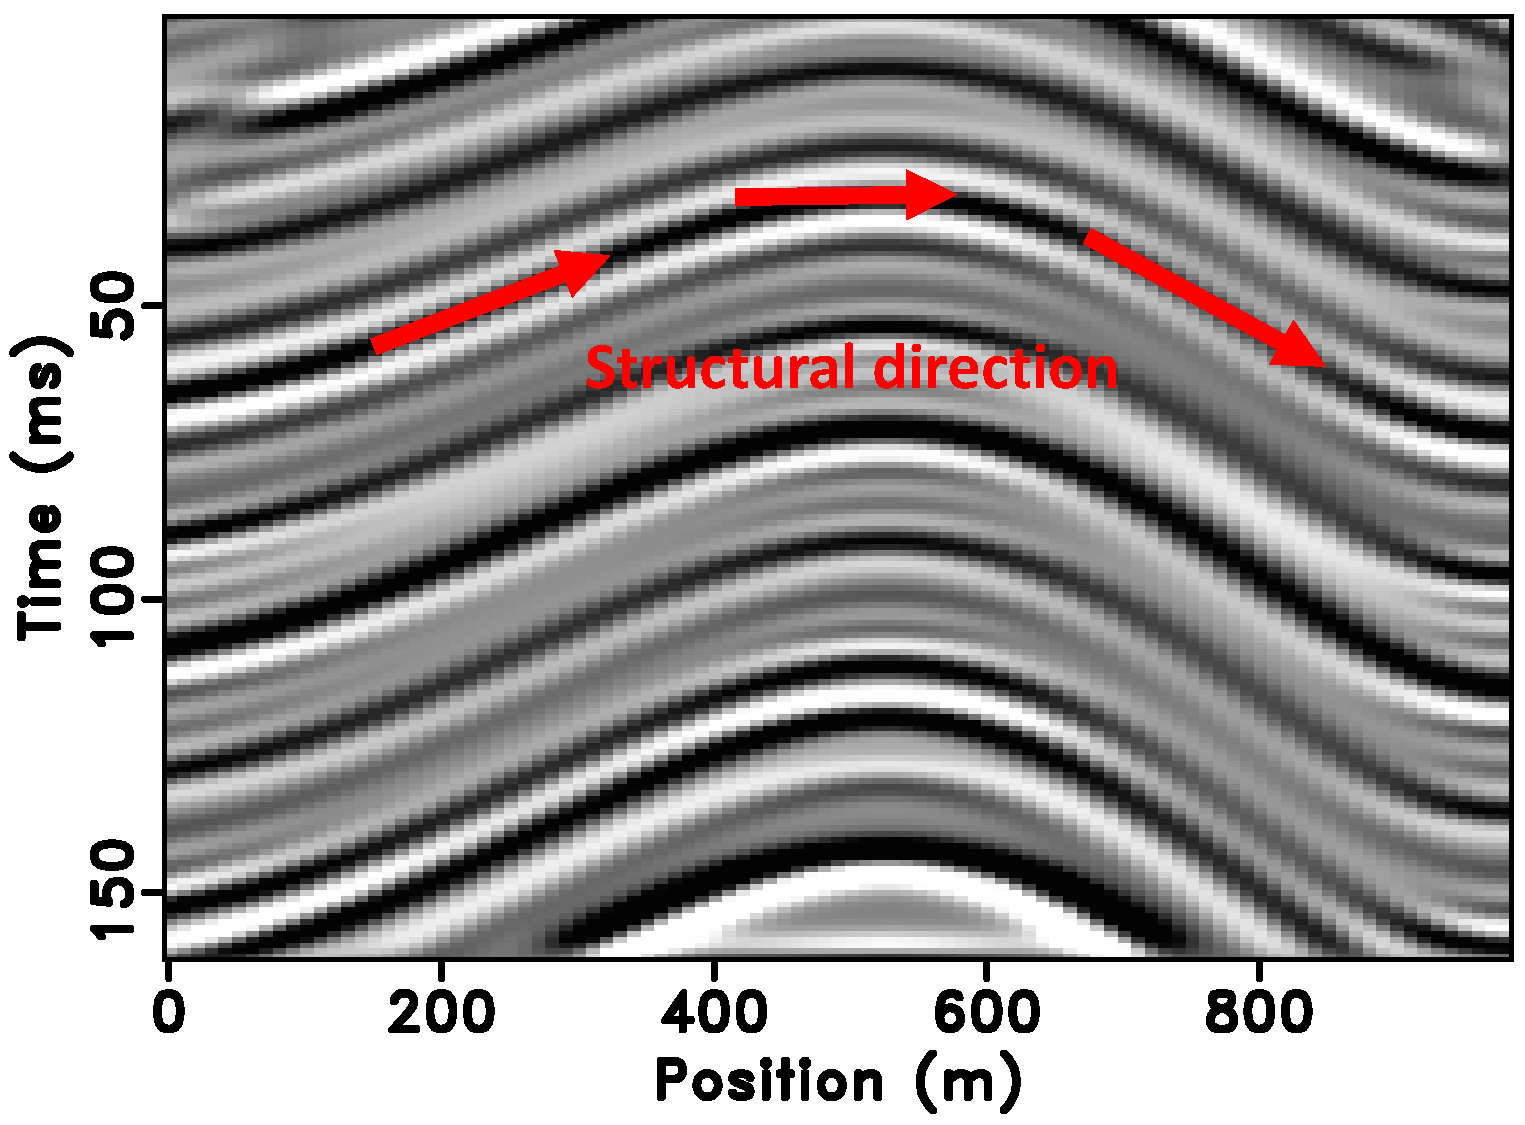
\includegraphics[width=0.5\columnwidth]{Fig/synth0}
    \label{fig:synth0}}  \\
  \subfloat[]{\includegraphics[width=0.5\columnwidth]{jy/Fig/synth-cube}
    \label{fig:synth-cube}}          
   \caption{A simple demonstration of structure-oriented processing. (a) Input data. (b) Locally flattened domain. The 2D section defined by the axes ``Time (ms)'' and ``Position (m)'' indicates the original profile so it contains curving events. The 2D section defined by the axes ``Time (ms)'' and ``\dlo{Position (m)}\wen{Prediction (trace)}'' indicates the flattened data. \wen{The 2D section defined by the axes ``Prediction (trace)'' and ``Position (m)'' indicates the constant Time slice.} }
   \label{fig:synth0,synth-cube}
\end{figure}

\begin{figure}[htb!]
  \centering
  \subfloat[]{\includegraphics[width=0.25\columnwidth]{jy/Fig/synth}
    \label{fig:sig}}  
  \subfloat[]{\includegraphics[width=0.25\columnwidth]{jy/Fig/dip}
    \label{fig:dip}} 
  \subfloat[]{\includegraphics[width=0.4\columnwidth]{jy/Fig/synth-cube}
    \label{fig:synths-cube}} \\    
  \subfloat[]{\includegraphics[width=0.25\columnwidth]{jy/Fig/synth-n}
    \label{fig:sig-n}} 
  \subfloat[]{\includegraphics[width=0.25\columnwidth]{jy/Fig/dip-n}
    \label{fig:dip-n}}   
  \subfloat[]{\includegraphics[width=0.4\columnwidth]{jy/Fig/synths-cuben}
    \label{fig:synths-cuben}}           
   \caption{(a) Clean data. (b) Slope estimated from (a). (c) Flattened domain of (a). (d) Noisy data. (e) Slope estimated from (d). (f) Flattened domain of (d).}
   \label{fig:sig,dip,synth-cube,sig-n,dip-n,synths-cube}
\end{figure}

\inputdir{jy}

\multiplot{6}{flat1,flat2,flat3,flat1-n,flat2-n,flat3-n}{width=0.29\textwidth}{A comparison of ``flattened" local windows (predicted dimension) for different space locations. (a)-(c) Flattened gathers for traces 9, 50, 90, using the accurate slope. (d)-(f) ``Flattened" gathers for traces 9, 50, 90, using the estimated slope.}

\inputdir{.}
\plot{svmf}{width=0.9\textwidth}{\wen{An illustration of the space-varying median filter. (a) Raw noisy data. (b) A map of constant filter length. (c) Initially filtered data using the constant filter length shown in (b). (d) Calculated local similarity map from (a) and (c) using equation \ref{eq:simi}. (e) Calculated map of variable filter length using equation \ref{eq:svmf2}. (f) Filtered data using the variable filter length shown in (e).}  }

\inputdir{jy}
\multiplot{6}{flat1-n-mf,flat2-n-mf,flat3-n-mf,flat1-n-svmf,flat2-n-svmf,flat3-n-svmf}{width=0.29\textwidth}{A denoising comparison of ``flattened" local windows (predicted dimension) using estimated slope for different space locations. (a)-(c) Denoised gathers for traces 9, 50, 90, using the \wen{median filter}. (d)-(f) \dlo{``Flattened"}\wen{Denoised} gathers for traces 9, 50, 90, using the \dlo{SVMF}\wen{space-varying median filter}. \wen{Note that although (c) is cleaner, the curving signals are serious damaged.}}

\multiplot{6}{flat1-n-mf-dif,flat2-n-mf-dif,flat3-n-mf-dif,flat1-n-svmf-dif,flat2-n-svmf-dif,flat3-n-svmf-dif}{width=0.29\textwidth}{\wen{A comparison of removed noise. (a)-(c) Removed noise for traces 9, 50, 90, using the median filter. (d)-(f) Removed noise for traces 9, 50, 90, using the space-varying median filter. Note that the median filter removes more coherent energy.}}


\inputdir{hyper}
\multiplot{4}{hyper,hyper-n,hdip,hdip-n}{width=0.4\textwidth}{(a) Clean data. (b) Noisy data with spike-like blending noise. (c) Estimated slope from the clean data. (d) Estimated slope from the noisy data. }

\multiplot{2}{hflat0,hflat-n0,hflat-n-mf0,hflat-n-svmf0}{width=0.45\textwidth}{(a) Flattened dimension of the clean data using the accurate slope. (b) Flattened dimension of the noisy data using the inaccurate slope. (c) Filtered data using \dlo{MF }\wen{median filter }in the flattened domain. (b) Filtered data using \dlo{SVMF}\wen{space-varying median filter} in the flattened domain.  }

\multiplot{2}{hflat-z0,hflat-n-z0,hflat-n-mf-z0,hflat-n-svmf-z0}{width=0.45\textwidth}{\wen{Zoomed comparison of Figure \ref{fig:hflat0,hflat-n0,hflat-n-mf0,hflat-n-svmf0}. (a) Flattened dimension of the clean data using the accurate slope. (b) Flattened dimension of the noisy data using the inaccurate slope. (c) Filtered data using median filter in the flattened domain. (b) Filtered data using space-varying median filter in the flattened domain. } }


\multiplot{4}{hyper-mf0,hyper-svmf0,hyper-somf0,hyper-sosvmf0}{width=0.38\textwidth}{(a) Deblended data using \dlo{MF}\wen{median filter}. (b) Deblended data using \dlo{SVMF}\wen{space-varying median filter}. (c) Deblended data using \dlo{SOMF}\wen{structure-oriented median filter}. (d) Deblended data using \dlo{SOSVMF}\wen{structure-oriented space-varying median filter}. \wen{Note that since all median filters are only applied once, so there are several spikes left. The one-step processing is efficient but can be improved through multiple iterations (e.g., in iterative deblending). }  }

\multiplot{4}{hyper-mf-z0,hyper-svmf-z0,hyper-somf-z0,hyper-sosvmf-z0}{width=0.4\textwidth}{\wen{Zoomed comparison of Figure \ref{fig:hyper-mf0,hyper-svmf0,hyper-somf0,hyper-sosvmf0}. (a) Deblended data using median filter. (b) Deblended data using space-varying median filter. (c) Deblended data using structure-oriented median filter. (d) Deblended data using structure-oriented space-varying median filter.}  }

\multiplot{4}{hyper-mf-n,hyper-svmf-n,hyper-somf-n,hyper-sosvmf-n}{width=0.35\textwidth}{(a)-(d) Removed blending noise sections corresponding to Figure\wen{s} \ref{fig:hyper-mf0,hyper-svmf0,hyper-somf0,hyper-sosvmf0} (a)-(c), respectively. }

\inputdir{field}
\multiplot{2}{shot-n,sdip-n}{width=0.48\textwidth}{(a) Simultaneous source data.  (b) Slope estimated from the raw data.  }

\multiplot{4}{shot-mf,shot-svmf,shot-somf,shot-sosvmf}{width=0.38\textwidth}{(a) Deblended data using \dlo{MF}\wen{median filter}. (b) Deblended data using \dlo{SVMF}\wen{space-varying median filter}. (c) Deblended data using \dlo{SOMF}\wen{structure-oriented median filter}. (d) Deblended data using \dlo{SOSVMF}\wen{structure-oriented space-varying median filter}.}

\multiplot{4}{shot-mf-n-0,shot-svmf-n-0,shot-somf-n-0,shot-sosvmf-n-0}{width=0.38\textwidth}{(a) Removed blending noise using \dlo{MF}\wen{median filter}. (b) Removed blending noise using \dlo{SVMF}\wen{space-varying median filter}.  (c) Removed blending noise using \dlo{SOMF}\wen{structure-oriented median filter}. (d) Removed blending noise using \dlo{SOSVMF}\wen{structure-oriented space-varying median filter}.}

\multiplot{4}{shot-mf-s,shot-svmf-s,shot-somf-s,shot-sosvmf-s}{width=0.38\textwidth}{A comparison of local similarity between deblended data and removed blending noise. (a) Local similarity using \dlo{MF}\wen{median filter}. (b) Local similarity using \dlo{SVMF}\wen{space-varying median filter}.  (c) Local similarity using \dlo{SOMF}\wen{structure-oriented median filter}. (d) Local similarity using \dlo{SOSVMF}\wen{structure-oriented space-varying median filter}.}


\section{Examples}
%In this section, we not only show the performance of the SOSVMF in attenuating blending noise
%that results from the simultaneous source acquisition, we also show an example on rejecting general spike-like noise. 

%We first test the performance of the SOSVMF in attenuating general spike-like noise. 
We first test the \dlo{SOSVMF}\wen{structure-oriented space-varying median filter} method on a simple synthetic example. Figure \ref{fig:hyper} shows a simple hyperbolic synthetic example. \wen{We create the data using the Kirchhoff 2-D/2.5-D modeling method with analytical Green's functions, introduced in \cite{haddon1981use}.} Figure \ref{fig:hyper-n} shows the noisy data with some
blending noise. Figure \ref{fig:hdip} shows the slope estimated from the clean data and Figure \ref{fig:hdip-n} shows the slope estimated from the noisy data. The strong noise makes the slope estimation inaccurate. Figures \ref{fig:hflat0} and \ref{fig:hflat-n0} show a comparison between the flattened unblended data using accurate slope and flattened blended data using inaccurate local slope, respectively. From Figure \ref{fig:hflat0}, we can observe that the data is flattened well locally using the accurate local estimation (from the unblended data). From Figure \ref{fig:hflat-n0}, it is obvious that the events in the flattened dimension are not horizontal, which indicates an imperfect local flattening.  Figures \ref{fig:hflat-n-mf0} and \ref{fig:hflat-n-svmf0} show a comparison between the filtered data using the \dlo{MF }\wen{median filter }and \dlo{SVMF}\wen{space-varying median filter}, respectively. Both \dlo{MF }\wen{median filter }and \dlo{SVMF}\wen{space-varying median filter} are applied along the flattened dimension (along the ``prediction'' axis). It is clear that some energy is damaged using the \dlo{MF }\wen{median filter }and the signals are preserved well using the \dlo{SVMF}\wen{space-varying median filter} method, as indicated by the white arrow in Figure \ref{fig:hflat0,hflat-n0,hflat-n-mf0,hflat-n-svmf0}. \wen{For a clearer comparison, we show the zoomed data of Figure \ref{fig:hflat0,hflat-n0,hflat-n-mf0,hflat-n-svmf0} in Figure \ref{fig:hflat-z0,hflat-n-z0,hflat-n-mf-z0,hflat-n-svmf-z0}.} Figure \ref{fig:hyper-mf0,hyper-svmf0,hyper-somf0,hyper-sosvmf0} shows a deblending comparison between the \dlo{MF,}\wen{median filter,} \dlo{SVMF}\wen{space-varying median filter}, \dlo{SOMF}\wen{structure-oriented median filter}, and \dlo{SOSVMF}\wen{structure-oriented space-varying median filter} methods, respectively. From Figure \ref{fig:hyper-mf0,hyper-svmf0,hyper-somf0,hyper-sosvmf0}, we can see that the traditional \dlo{MF }\wen{median filter }results in the \dlo{lagest}\wen{largest} damages, which is followed by \dlo{SVMF}\wen{space-varying median filter}. \dlo{SOMF}\wen{structure-oriented median filter} preserves most signals but still causes some damages, as indicated by the white arrow. Among the four results, the \dlo{SOSVMF}\wen{structure-oriented space-varying median filter} result is the best in preserving dipping energy and rejecting spike-like blending noise. \wen{A zoomed comparison of Figure \ref{fig:hyper-mf0,hyper-svmf0,hyper-somf0,hyper-sosvmf0} is shown in Figure \ref{fig:hyper-mf0,hyper-svmf0,hyper-somf0,hyper-sosvmf0}.} Figure \ref{fig:hyper-mf-n,hyper-svmf-n,hyper-somf-n,hyper-sosvmf-n} shows the removed blending noise corresponding to the four aforementioned methods, which confirms the observation from Figure \ref{fig:hyper-mf0,hyper-svmf0,hyper-somf0,hyper-sosvmf0} that \dlo{MF,}\wen{median filter,} \dlo{SVMF}\wen{space-varying median filter}, and \dlo{SOMF}\wen{structure-oriented median filter} all result in more or less signal leakage \cite[]{yangkang2015ortho} to the noise sections. In this example, we use the signal-to-noise ratio (SNR) to quantitatively compare the deblending performance using different methods:
\begin{equation}
\label{eq:diff}
SNR=10\log_{10}\frac{\Arrowvert \mathbf{m}_{clean} \Arrowvert_2^2}{\Arrowvert \mathbf{m}_{clean} -\mathbf{m}\Arrowvert_2^2},
\end{equation}
where $\mathbf{m}_{clean}$ denotes the exact solution, or the unblended data. $\mathbf{m}$ denotes the deblended data. Using this metic, we calculate the SNRs of the blended data, deblended data using \dlo{MF,}\wen{median filter,} \dlo{SVMF}\wen{space-varying median filter}, \dlo{SOMF}\wen{structure-oriented median filter}, and \dlo{SOSVMF}\wen{structure-oriented space-varying median filter} methods as 1.62 dB, 5.46 dB, 8.63 dB, 12.46 dB, and 16.55 dB, respectively. The \dlo{SOSVMF}\wen{structure-oriented space-varying median filter} method obtains the highest SNR.

The next example is a field data test. Figure \ref{fig:shot-n} shows the a common receiver gather that contains blending noise. \wen{The data is a benchmark testing data shared by BGP, China.} Figure \ref{fig:sdip-n} shows the local slope map calculated from the raw data using the \dlo{PWD}\wen{plane-wave destruction} algorithm. The deblended results using four methods are shown in Figure \ref{fig:shot-mf,shot-svmf,shot-somf,shot-sosvmf}. The removed blending noise corresponding to the four methods are shown in Figure \ref{fig:shot-mf-n-0,shot-svmf-n-0,shot-somf-n-0,shot-sosvmf-n-0}. Combining Figures \ref{fig:shot-mf,shot-svmf,shot-somf,shot-sosvmf} and \ref{fig:shot-mf-n-0,shot-svmf-n-0,shot-somf-n-0,shot-sosvmf-n-0}, it is easy to conclude that both \dlo{MF }\wen{median filter }and \dlo{SVMF}\wen{space-varying median filter} methods cause a large amount of damaged energy, the \dlo{SOMF}\wen{structure-oriented median filter} method causes relatively less damaged energy around the large-offset areas, and the \dlo{SOSVMF}\wen{structure-oriented space-varying median filter} method causes negligible damaged energy. Note that the signal damages are highlighted by the white arrows in Figure \ref{fig:shot-mf-n-0,shot-svmf-n-0,shot-somf-n-0,shot-sosvmf-n-0}. In this example, the exact solution is unknown, thus we cannot use the quantitative metric that is used previously to compare the performance quantitatively. But we use the local similarity to measure the signal damage. The local similarity between the denoised (deblended) and removed noise sections are calculated to detect the signal damage for a denoising (deblending) algorithm, as proposed in \cite{yangkang2015ortho}. High anomalies in the local similarity map indicates a more servere signal damage. The most distinct advantage of the local similarity measure is that it can measure the signal damage in a local and vivid way. Figure \ref{fig:shot-mf-s,shot-svmf-s,shot-somf-s,shot-sosvmf-s} show the four local similarity maps for the four methods. The comparison of local similarity shows vividly that all \dlo{MF,}\wen{median filter,} \dlo{SVMF}\wen{space-varying median filter}, and \dlo{SOMF}\wen{structure-oriented median filter} methods cause a large amount of damaged signals in the noise and the signal damage using the \dlo{SOSVMF}\wen{structure-oriented space-varying median filter} method is the least. \wen{It is worth mentioning that some shallow reflections are not well predicted.  This is likely because of the curvature of the events and the linearity of the process.}

Next, we simulate a multi-receivers 2D simultaneous source separation test. In this test, we want to test how the \dlo{SOSVMF}\wen{structure-oriented space-varying median filter} method performs when embedded into an iterative deblending framework. Figure \ref{fig:geom} shows the acquisition geometry of the 2D test. The red dots denote 120 evenly spaced shot locations on the surface. \dlo{The red strings denote the ray paths underneath the surface.} The blue inverted triangles denote 120 evenly spaced receivers. Note that in this acquisition geometry, the simultaneous shooting and traditional shooting only differ in the shot schedule \cite[]{abma2014}. Figure \ref{fig:shottime} shows the shot schedules for the traditional and the faster simultaneous source shooting. It is worth mentioning here that although there is only one source in this test, the faster shooting scheduling results in an overlapping subsurface reflection responses in time, which is still considered as simultaneous shooting \cite[]{abma2015}. From the shot schedule, it is obvious that the shooting time for the simultaneous source acquisition is almost half of the traditional acquisition and thus saves about half of the traditional acquisition cost. In this example, we use a relatively realistic field dataset to mimic the unblended data ($\mathbf{m}$ in equation \ref{eq:blend}), as shown in Figure \ref{fig:d3d}. \wen{The data is a marine data set provided by BGP China.} The size of the data is $1500\times 120\times120$ \wen{(in time-shot-receiver domain)}. Figure \ref{fig:b3d} shows the blended data ($\mathbf{d}$ in equation \ref{eq:blend}). It is clear that the blending noise appears to be spatially incoherent in the common receiver domain (along the shot axis) and spatially coherent in the common shot domain (along the receiver axis). Figure \ref{fig:m3d} shows iteratively deblended data using the rank-constrained shaping regularization framework \dlo{(equation \ref{eq:iter})} \cite[]{yangkang20142,shaohuan2017gji}. The iterative deblending is carried out in each common receiver gather based on the coherency difference between useful signals and interfering noise. For the rank-constrained inversion, we use local windows with the size of $200\times 20$ \wen{($\text{time} \times \text{space}$)}. A constant rank strategy is used for each window with $rank=2$. We obtain the result shown in Figure \ref{fig:m3d} with 40 iterations. Comparing the rank-constrained deblended data with the blended data, it is clear that most blending noise is removed. However, there is still \dlo{a lot of}\wen{much} residual noise. By cascading the \dlo{SOSVMF}\wen{structure-oriented space-varying median filter}\dlo{ filter} and the rank filter based on the iterative shaping regularization framework, as expressed by equations \ref{eq:iter}, we obtain a much improved deblended result, as shown in Figure \ref{fig:im3d}. During the inversion, we linearly decrease the filter length from 11 points to 0. A comparison between the two deblended data in Figure \ref{fig:m3d,im3d} confirms the effectiveness of the \dlo{SOSVMF}\wen{structure-oriented space-varying median filter} method in improving iterative deblending. Figure \ref{fig:m3d-e,im3d-e} shows the deblending error for the traditional method and the proposed method. The deblending error means the difference between the unblended data (exact solution) and the deblended data. From Figure \ref{fig:m3d-e,im3d-e}, it is obvious that the deblending error for the proposed method is negligible while the error for the \dlo{traditional}\wen{rank-reduction} method is very large. Figure \ref{fig:m3d-n,im3d-n} shows the removed noise corresponding to the two methods\wen{, note that the interfering shots are coherent in the second spatial dimension.}. For evaluating the signal damages of this example, we calculate the local similarity between the deblended data and \dlo{removed}\wen{the} noise and show them in Figure \ref{fig:m3d-s,im3d-s}, where much larger local similarity anomalies are shown in the similarity map corresponding the traditional method. To compare the amplitude preservation in detail, we plot a trace-by-trace comparison in Figure \ref{fig:trace}. The black line is from the unblended data. The red line is from the blended data. The \dlo{blue}\wen{magenta} line corresponds to the rank-constrained method. The green line corresponds to the proposed \dlo{SOSVMF-rank-constrained }method. It is salient that the black and green lines are very close to each other, thus the deblending error using the proposed approach is much less than the traditional method for most parts. \wen{In order to compare the hybrid method with the structure-oriented space-varying median filter and the hybrid with the structure-oriented median filter, we also have a inversion test using the structure-oriented median filter. The deblended data is shown in Figure \ref{fig:im3d-2,im3d-e-2}. It is obvious that the hybrid method with the structure-oriented median filter causes much higher deblending error. }


\inputdir{./}
\multiplot{2}{geom,shottime}{width=0.5\textwidth}{(a) Acquisition geometry. \dlo{The red strings denote the ray paths underneath the surface.} The red dots denote shot locations and blue inverted triangles denote receivers. The simultaneous shooting and the traditional shooting only differ in the shot schedule. (b) Shot schedule. Note that the shot schedule is just for testing purpose and does not represent a real field deployment. In the test, the speed of a shooting vessel is assumed to be sufficiently large. In practice, the shot sampling would be much higher than the testing case, which is 0.05 km.}


\multiplot{2}{d3d,b3d}{width=0.6\textwidth}{Shot-receiver data example. (a) Unblended data. (b) Blended data.}
\multiplot{2}{m3d,im3d}{width=0.6\textwidth}{A comparison between \wen{iterative} deblending performance. (a) \dlo{Traditionally}\wen{Iteratively} deblended data using the rank-constrained method. (b) Deblended data using the \dlo{SOSVMF-rank-constrained}\wen{proposed} method.}

\multiplot{2}{m3d-e,im3d-e}{width=0.6\textwidth}{A comparison between deblending error. (a) Error corresponding to the traditional rank-constrained method. (b) Error corresponding to the \dlo{SOSVMF-rank-constrained}\wen{proposed} method.}

\multiplot{2}{m3d-n,im3d-n}{width=0.6\textwidth}{A comparison between removed blending noise. (a) Removed blending noise corresponding to the traditional rank-constrained method. (b) Removed blending noise corresponding to the \dlo{SOSVMF-rank-constrained}\wen{proposed} method.}

\multiplot{2}{m3d-s,im3d-s}{width=0.5\textwidth}{A comparison between local similarity comparison. (a) Local similarity corresponding to the traditional rank-constrained method. (b) Local similarity corresponding to the \dlo{SOSVMF-rank-constrained}\wen{proposed} method. Note the much larger similarity anomaly shown in (a).}

\multiplot{2}{trace,trace-z}{width=0.5\textwidth}{Single trace comparison. The black line is from the unblended data. The red line is from the blended data. The \dlo{blue}\wen{magenta} corresponds to the rank-constrained method. The green line corresponds to the proposed \dlo{SOSVMF-rank-constrained}\wen{proposed} method. Note that the black and green lines are very close to each other, thus the deblending error using the proposed approach is much less than the traditional method for most parts. \wen{(a) Comparison in the original size. (b) Comparison in a zoomed view.}}

\multiplot{2}{im3d-2,im3d-e-2}{width=0.5\textwidth}{\wen{Deblending performance using the hybrid method with structure-oriented median filter. (a) Deblended data. (b) Deblending error. Note that the deblending error in this case is much higher than the hybrid method with structure-oriented space-varying median filter (Figure \ref{fig:im3d-e}).}}

\wen{\section{Discussion}}
\wen{Two main research tracks of deblending are the filtering method, which is fast and easy to control, and the inversion method, which is more computationally demanding but can obtain better result. Two main existing challenges for deblending are 1) damaging signals for the filtering method and 2) lacking extra constraints during inversion in order to deal with high blending fold \cite[]{arazthesis2012}. The paper mainly discusses the filtering based deblending methods, so let us first focus on the drawbacks of the filtering method. To date, the filtering based deblending methods are mainly based on some types of median filtering, e.g., \cite{mediandeblend}, \cite{yangkang2015svmf}, \cite{shuwei2016}, and etc. Median filtering is a classic method. However, when we dig into the median filtering method further and further, we find that the implementation of a traditional median filter affects the result significantly. For example, \cite{mediandeblend} propose to apply the median filter to the dip direction of the seismic events, which can preserve the useful energy well. \cite{yangkang2015svmf} proposes to apply the median filter with different filter lengths, which can also preserve the useful energy well. \cite{shuwei2016} propose a similar method  as \cite{mediandeblend} but with a different structural filtering strategy and a different slope/dip estimation strategy. However, both \cite{mediandeblend}  and \cite{shuwei2016} depend  on accurate slope/dip estimation. What if slope/dip is not estimated accurately, e.g., in extremely noisy blended data or not in CMP gathers (as required by \cite{shuwei2016})? Then, both methods fail. In addition, for \cite{yangkang2015svmf}'s method, what if there exists steeply dipping events? No matter what thresholds of the method we use, it fails. The structure-oriented space-varying median filter is not a seemingly simple concatenation. It relieves the influence of slope/dip estimation on the following median filtering (traditional). So the dependency of an accurate slope/dip estimation no longer exists. Besides, because of the flattening (or approximate flattening when slope/dip is not accurate), the events are guaranteed to be not steeply dipping. The combination of the two methods is elegant, which solves two long-existing and fundamental problems for the ``median filtering'' based deblending  methods. The straightforward benefit is that we can deal with the massive blended data in a very fast and amplitude-preserving way.}

%First, we would like to discuss the computational cost of the SOSVMF filter. 
The \dlo{SOSVMF}\wen{structure-oriented space-varying median filter} is not computationally expensive. To understand the computational cost of the \dlo{SOSVMF}\wen{structure-oriented space-varying median filter} better, we can first split \dlo{SOSVMF}\wen{structure-oriented space-varying median filter} into two components: \dlo{SVMF}\wen{space-varying median filter} and \dlo{SOMF}\wen{structure-oriented median filter}. Compared with the traditional \dlo{MF}\wen{median filter}, the \dlo{SVMF}\wen{space-varying median filter} uses a \dlo{MF}\wen{median filter} twice, each with different filter length criterion, thus the computational cost of \dlo{SVMF}\wen{space-varying median filter} is about the twice of the cost of the \dlo{MF}\wen{median filter} plus the calculation of the local similarity between the initially filtered data and a removed noise section. Calculation of the local similarity is also an efficient algorithm thanks to the fast implementation of the shaping regularization framework \cite[]{fomel2007localattr}. The \dlo{SOMF}\wen{structure-oriented median filter} adds an extra flattening (or trace prediction) step into the traditional \dlo{MF}\wen{median filter} and the extra computational cost is composed of local slope calculation and spatial neighbor trace prediction. According to our experience, the 2D calculation is still acceptable. More details of slope calculation are referred to \cite{fomel2002pwd} and more explanations regarding the trace prediction can be found in \cite{liuyang2010}. The main computational cost of \dlo{SOSVMF}\wen{structure-oriented space-varying median filter} comes from calculation of the local slope, trace prediction, and local similarity calculation required by \dlo{SVMF}\wen{space-varying median filter} in each flattened local gather. All these extra computational steps can be implemented via efficient algorithms based on shaping regularization \cite[]{fomel2007shape}, thus the application of the \dlo{SOSVMF}\wen{structure-oriented space-varying median filter} is not expensive. Here, we compare the computational cost in time for four different filtering methods in Table \ref{tbl:time}. The computation is done on a PC station equipped with an Intel Core i7 CPU clocked at 3.1 GHz and 16 GB of RAM. With a small data size, the computational cost for four methods are comparable. For a large data size (e.g., $800 \times 400$), the computational cost for the \dlo{SOSVMF}\wen{structure-oriented space-varying median filter} is roughly 3 times that of the \dlo{SOMF}\wen{structure-oriented median filter}. It is also worth noting that the actual calculation time is usually data dependent. The exact calculation time for the local slope estimation and similarity computation may vary according to the input data but are not expensive. 

%\tabl{time}{Comparison of computational time. MF denotes median filter. SVMF denotes space-varying median filter. SOMF denotes structure-oriented median filter. SOSVMF denotes structure-oriented space-varying median filter. }
% {

%} 

The \dlo{SOSVMF}\wen{structure-oriented space-varying median filter} is close to an adaptive method. The only parameter that needs to be chosen is the filter length. Once the filter length $L$ is fixed, the filter can adaptively adjust according to the complicated seismic structure via the two-step cascaded structure-oriented filtering and variable window strategy. Traditionally, the performance of the structure-oriented filtering highly depends on the local slope calculated from the noisy data. While adjusting the the parameters for the \dlo{PWD}\wen{plane-wave destruction} algorithm, e.g., the smoothing radius, regularization parameters, and the number of iterations, can somewhat improve the performance of slope estimation, it is still almost impossible to output an optimal slope map. As shown in the beginning part of the paper, a roughly calculated local slope map will result in unflattened local gathers and are not suitable for a simple median filtering. The \dlo{SOSVMF}\wen{structure-oriented space-varying median filter} eases the dependency of the performance on the input slope field in that the following \dlo{SVMF}\wen{space-varying median filter} can deal with the unflattened energy via the variable window strategy. From a different aspect, the traditional \dlo{SVMF}\wen{space-varying median filter} does not account for the structure patterned existing in seismic data and is only effective to events with smaller dip angle. The local flattening process in structural filtering helps the \dlo{SVMF}\wen{space-varying median filter} prepare events with small dip angle. Combining the strategies of structural filtering and variable window length, the \dlo{SOSVMF}\wen{structure-oriented space-varying median filter} \dlo{is almost adaptive to any}\wen{is adaptive to almost any} input data with an arbitrary level of structural complexity. \new{For example, in the supplementary data, we show the results of a crossing-event dataset, where we can find that the proposed method also adapts to dataset containing crossing events.}


%Secondly, parameterization of the SOSVMF is not not complicated. 
\dlo{The SOSVMF is not limited to seismic data processing. Due to the strong signal-preserving ability of SOSVMF, it has the potential to be widely applied to remove spike-like noise in any type of datasets that contain structural patterns. Here, we want to mention an interesting application of the SOSVMF method in improving the waveforms recorded from the laser interferometor, which is usually used to study the anisotropy of organic-rich shale in rock physics. 
The laser ultrasonic approach has outstanding advantages in measuring elastic and anisotropic parameters and seismic physical modeling compared with the transducers ultrasonic approach in (1) no coupling and ring problems, (2) denser sampling, (3) fast and automatic acquisition, (4) exact group velocity.  The principle is to obtain the waveforms in each direction to the bedding plane in a horizontal cored shale sample, from which we can acquire a large number of diagonal group velocities versus group angle to invert the elastic constants and anisotropic parameters.  However, due to the extreme complexity of diagenetic overprints (temperature, overlying pressure, time), lithology and intrinsic properties (porosity, permeability, mineral components, etc) of organic-rich shale, the conversion efficiency of laser-ultrasonic is usually too low to be discerned when the laser pulse hits the surface of sample directly, which makes it difficult to obtain signals with high signal-to-noise ratio (SNR). Figure ? shows a recorded data from the  laser interferometor, which contains significant amount of noise. Figure ? shows the denoised data using the proposed SOSVMF method, and Figure ? shows the corresponding removed noise, which is generally spatially incoherent and does not contain obvious useful waveform signal.}
%The SOSVMF is not limited to seismic data processing. Due to the strong signal-preserving ability of SOSVMF, it has the potential to be widely applied to remove spike-like noise in any type of datasets that contain structural patterns. Here, we want to mention an interesting application of the SOSVMF method in improving the waveforms recorded from the laser interferometor, which is usually used to study the anisotropy of organic-rich shale in rock physics. The laser ultrasonic approach has outstanding advantages in measuring elastic and anisotropic parameters \cite[]{Aussel1989, Pouet1993,Lebedev2011, Carson2014} and seismic physical modeling \cite[]{blum2010, Bretaudeau2011} compared with the transducers ultrasonic approach in (1) no coupling and ring problems, (2) denser sampling, (3) fast and automatic acquisition, (4) exact group velocity \cite[]{blum2013,jianyong2016}.  The principle is to obtain the waveforms in each direction to the bedding plane in a horizontal cored shale sample, from which we can acquire a large number of diagonal group velocities versus group angle to invert the elastic constants and anisotropic parameters.  However, due to the extreme complexity of diagenetic overprints (temperature, overlying pressure, time), lithology and intrinsic properties (porosity, permeability, mineral components, etc) of organic-rich shale, the conversion efficiency of laser-ultrasonic is usually too low to be discerned when the laser pulse hits the surface of sample directly, which makes it difficult to obtain signals with high signal-to-noise ratio (SNR). Figure \ref{fig:data} shows a recorded data from the laser interferometor, which contains significant amount of noise. Figure \ref{fig:data-somf} shows the denoised data using the proposed SOSVMF method, and Figure \ref{fig:data-somf-n} shows the corresponding removed noise, which is generally spatially incoherent and does not contain obvious useful waveform signal.

%\inputdir{laser}
%\multiplot{3}{data,data-somf,data-somf-n}{width=0.7\textwidth}{(a) Recorded data from the laser interferometor. (b) Denoised data using the SOSVMF method. (c) Removed noise using the SOSVMF method.}

\section{Conclusion}
The signal preserving ability of a median filter\dlo{ (MF)} has been improved from the classic implementation to a space-varying median filter\dlo{ (SVMF)}, and further to a structure-oriented median filter\dlo{ (SOMF)}. However, the performance of \dlo{SOMF}\wen{structure-oriented median filter} highly depends on the accuracy of \dlo{the }estimated local slope\wen{s} of the input seismic data. We have proposed a variant of MF\wen{, named structure-oriented space-varying median filter,} that preserves signal energy even in \wen{cases with} complicated structure\wen{,} and can adapt to the inaccurate slope estimation in a structure-oriented filtering framework by applying a \dlo{SVMF}\wen{space-varying median filter} along the imperfectly flattened dimension. The proposed \dlo{SOSVMF }method can be applied to \dlo{reject}\wen{remove} spike-like noise in datasets that contain structural patterns. \dlo{The application of the SOSVMF in simultaneous source separation demonstrates a successful performance and shows distinct advantages over traditional alternative MFs.} \dlo{SOSVMF}\wen{Structure-oriented space-varying median filter} can also be conveniently used as an extra constraint during iterative deblending to improve the deblending performance based on the shaping regularization framework. Both synthetic and field data examples demonstrate the great advantages and potential of the \dlo{SOSVMF}\wen{the proposed method}.


\section{Acknowledgements}
The authors would like to thank Sergey Fomel, Shan Qu, Yaru Xue, Wei Chen, Min Bai, Dong Zhang, Jianyong Xie, Josef Paffenholz, Araz Mahdad, Ray Abma, Min Zhou, Qie Zhang, \wen{and} Zhiyong Jiang for \dlo{better }inspiring discussions on the simultaneous source separation problem. Yangkang Chen \dlo{is appreciated to}\wen{appreciates} FairfieldNodal and BP America for offering \dlo{his }summer internships during his PhD study at UT Austin. %The authors also thank editors Jeffrey Shragge and Guy Drijkoningen, reviewer Ying Wang, and \wen{three} other anonymous reviewers for constructive comments.  
\new{The authors also thank Herve Chauris, S.Mostafa Mousavi, and an anonymous reviewers for constructive comments.} The research is partially supported by \wen{the “Thousand Youth Talents Plan”, the starting fund from Zhejiang University, }National Natural Science Foundation of China (Grant No. U1262207), National Engineering Laboratory of Offshore Oil Exploration, 973 Program of China (Grant No. 2013CB228603), \wen{and} the National Science and Technology Program (Grant No. 2016ZX05010002-002).


\section{Appendix: Local similarity}
 Local similarity between vectors $\mathbf{a}$ and $\mathbf{b}$ is defined as:
\begin{equation}
\label{eq:local}
\mathbf{c}=\sqrt{\mathbf{c}_1\circ\mathbf{c}_2},
\end{equation}
where $\circ$ denotes element-wise product\dlo{,}\wen{.} $\mathbf{c}_1$ and $\mathbf{c}_2$ come from two least-squares minimization problems:
\begin{align}
\label{eq:local1}
&\min_{\mathbf{c}_1}\Arrowvert \mathbf{a}-\mathbf{B} \mathbf{c}_1 \Arrowvert_2^2, \\
\label{eq:local2}
&\min_{\mathbf{c}_2}\Arrowvert \mathbf{b}-\mathbf{A} \mathbf{c}_2 \Arrowvert_2^2.
\end{align}
\dlo{where}\wen{Here,} $\mathbf{A}$ is a diagonal operator composed of the elements of $\mathbf{a}$, $\mathbf{B}$ is a diagonal operator composed of the elements of $\mathbf{b}$. Note that in equations \ref{eq:local}-\ref{eq:local2}, $\mathbf{a}$, $\mathbf{b}$, and $\mathbf{c}$  denote vectorized 2D matrices. Equations \ref{eq:local1} and \ref{eq:local2} can be solved using shaping regularization with a local-smoothness constraint:
\begin{align}
\label{eq:local3}
\mathbf{c}_1 &= [\lambda_1^2\mathbf{I} + \mathbf{T}(\mathbf{B}^T\mathbf{B}-\lambda_1^2\mathbf{I})]^{-1}\mathbf{TB}^T\mathbf{b},\\
\label{eq:local4}
\mathbf{c}_2 &= [\lambda_2^2\mathbf{I} + \mathbf{T}(\mathbf{A}^T\mathbf{A}-\lambda_2^2\mathbf{I})]^{-1}\mathbf{TA}^T\mathbf{a},
\end{align}
where $\mathbf{T}$ is a smoothing operator\dlo{ and}\wen{,} $\lambda_1$ and $\lambda_2$ are two parameters controlling the physical dimensionality and enabling fast convergence when inversion\wen{s} \wen{for $\mathbf{c}_1$ and $\mathbf{c}_2$ expressed in equations \ref{eq:local3} and \ref{eq:local4}} are implemented iteratively. \wen{$\lambda_1$ and $\lambda_2$} can be chosen as $\lambda_1  = \Arrowvert\mathbf{B}^T\mathbf{B}\Arrowvert_2$ and $\lambda_2  = \Arrowvert\mathbf{A}^T\mathbf{A}\Arrowvert_2$.






\bibliographystyle{seg}
\bibliography{mf}

\newpage
\listoftables
\newpage
\begin{table}[!ht]
\caption{Comparison of computational time. MF denotes median filter. SVMF denotes space-varying median filter. SOMF denotes structure-oriented median filter. SOSVMF denotes structure-oriented space-varying median filter.}
    \begin{center}
     \begin{tabular}{|c|c|c|c|c|} 
	  \hline Model size & 50$\times$50  &  100$\times$100 & 200$\times$200 & 800$\times$ 400\\ 
	  \hline MF (s) & 0.442 & 0.460 & 0.471 & 0.591\\
      \hline SVMF (s) & 0.473	& 0.491	   & 0.527   & 0.962	 \\ 
      \hline SOMF (s) & 0.491 & 0.508 	&0.600	 & 1.525\\
      \hline SOSVMF (s) & 0.660  & 0.848 	&1.769	 & 4.237\\
      \hline
    \end{tabular} 
   \end{center}
   \label{tbl:time}
\end{table}








